\documentclass[../VorlesungMaster.tex]{subfiles}

%Vorlesung 7
%\section{Lineare Regressionsmodelle}
\section{Statistische Modelle}
Lineare Regressionsmodelle:
\begin{itemize}
	\item Einfache lineare Regressionsmodelle
	\item Multivariate lineare Regressionsmodelle
	\item Voraussetzungen für lineare Regressionsmodelle
	\item Generalisierte lineare Regressionsmodelle (GLM)
	\item Auswertung von Expressionsdaten
\end{itemize}
Molekularbiologische Hochdurchsatzdaten:\\
\begin{center}
	\begin{tikzpicture}
	\node[fill=white,
	thick,
	draw,
	minimum height=3.5cm,
	minimum width=1.5cm
	](n1){};
	\node[left=0cm of n1](t1){\# Elemente $\downarrow$};
	\node[above=0cm of n1](t2){$\rightarrow$ \# Sample};
	\end{tikzpicture}
\end{center}

\#Elemente $>>$ \#samples\\
\begin{itemize}
	\item Genom $\rightarrow$ SNP
	\item Epigenom
	\item \underline{Transkriptom} $\rightarrow$ RNA Content einer Zelle
\end{itemize}

\begin{center}
	\begin{tikzpicture}
	\node[fill=white,
	thick,
	draw,
	minimum height=0.5cm,
	minimum width=1.0cm,
	](n1){};
	\node[fill=white,
	right=1cm of n1,
	thick,
	draw,
	minimum height=0.5cm,
	minimum width=1.0cm,
	](n2){};
	\node[fill=white,
	right=1cm of n2,
	thick,
	draw,
	minimum height=0.5cm,
	minimum width=1.0cm,
	](n3){};
	\node[fill=white,
	right=1cm of n3,
	thick,
	draw,
	minimum height=0.5cm,
	minimum width=1.0cm,
	](n4){};
	
	\node[below=1cm of n1,xshift=5cm](text1){pre-m-RNA $\rightarrow$ ncRNA $\rightarrow$ mRNA $\rightarrow$ Protein};
	\node[below=0.1cm of n4](text2){Exons};
	\node[right=0.5cm of n4](text3){DNA};
	
	\draw [] (-1,0) edge (n1);
	\draw [] (n1) edge (n2);
	\draw [] (n2) edge (n3);
	\draw [] (n3) edge (n4);
	\draw [] (7,0) edge (n4);
	
	\draw [->,thick] (n1) edge (text1.west);
	
	
	\end{tikzpicture}
\end{center}


\underline{Ziel}: Messen der Werte einer Zielvariablen in Abhängigkeit von unabhängigen Variablen (sog. Kovariaten) \\
\underline{Def}: Ein statistisches Model stellt eine Zielvariable $Y$ in Beziehung zu \underline{einer} oder mehreren Kovariaten (Kovariablen). \\
Zielvariable = Modell(Kovariate) + Fehler \\
\[ Y = f(X) + \epsilon \]
$Y$: Zielvariable oder auch abhängige Variable \\
$X$: Kovariaten oder auch unabhängige Variable \\
$f(X)$: Unbekannte Funktion, die den systematischen Effekt von $X$ auf $Y$ modelliert \\
$\epsilon$: Zufälliger Fehler. Gibt den Anteil der Varianz von $Y$ an, der \underline{nicht} durch $f(X)$ erklärt werden kann. \\
$\Rightarrow$ Statistische Modelle zerlegen die Zielvariable in einen systematischen ($f(X)$) und in einen zufälligen Teil ($\epsilon$). \\

\subsection{Anwendungen von statistischen Modellen}
Inferenz: Ziel ist es die Art des Zusammenhanges zwischen $Y$ und $X$ zu verstehen. Genauer: Wie ändert sich $Y$ als Funktion von $X$?\\
Vorhersage: Ziel ist es, den Wert von $Y$ so genau wie möglich vorherzusagen. Es ist nicht von primären Interesse die (exakte) Form von $f(X)$ zu kennen. \\

\subsection{Schätzen der Funktion $f(X)$}
$f(X)$ wird mittels einer statischen Lernmethode von einer Menge von Trainingsdaten geschätzt. Die geschätzte Funktion wird mit $\hat{f}(X)$ angegeben.
\[ Y = \hat{f}(X) + \epsilon \]
für Trainingsdaten $(X,Y) = \{(x_1,y_1),...,(x_n,y_n)\}$ n Beobachtungen.

\subsection{Klassifikation statistischer Lernmethoden}
\underline{Parametrische Methoden}: Für die Funktion $f(X)$ wird eine bestimmte Form angenommen.
\begin{enumerate}
	\item Anzahl der Kovariabln wird vorab festegelegt oder mittels Verfahren der Modellselektion ausgewählt.
	\item Es werden die Gewichte für die Kovariablen geschätzt
\end{enumerate}
Nachteil: 
\begin{enumerate}
	\item weniger flexibel
	\item Gewähltes Modell entspricht oft nicht der wahren Form des Zusammenhanges
\end{enumerate}
Vorteil:
\begin{enumerate}
	\item Da nur Gewichte für Kovariablen gelernt werden müssen, reicht eine geringe Stichprobengröße aus
\end{enumerate}

\underline{Nicht-parametrische Methoden}: Es wird keine bestimmte Form für $f(X)$ vorab angenommen.
Es muß die Form und die Parameter für eine beliebig komplexe Funktion $f(X)$ anhand der Trainingsdaten geschätzt werden.
Vorteil:
\begin{enumerate}
	\item Modelle sind sehr flexibel
\end{enumerate}

Nachteil:
\begin{enumerate}
	\item oft weniger gut interpretierbar
	\item oft ein großer Stichprobenumfang notwendig
\end{enumerate}

\section{Lineare Regressionsmodelle}
Als Form für $f(X)$ wird ein (annähernd) linearer Zusammenhang angenommen. Zufallsvariable $Y$ nimmt dabei quantitative Werte an. 
Kovariablen $X_i$ können quantitative oder qualitative Werte annehmen.

\subsection{Einfaches lineares Regressionsmodel}
\underline{Def.} Statistisches Modell, was den Wert der Zielvariablen $Y$ auf Basis der Werte einer einzigen Kovariable $X$, unter der Annahme eines linearen Zusammenhangs modelliert.

\[ Y = \underbrace{\beta_0 + \beta_1}_{Koeffizienten} + \epsilon \]
$\beta_0$: Mittelwert von $Y$, falls es keinen Zusammenhang gibt, sonst Schnittpunkt mit $y-Achse$. \\
$\beta_1$: \underline{Effekt} der Kovariablen $X$ auf $Y$ an, also den Anstieg in $Y$, wenn $X$ sich um eine Einheit erhöht. (Regressionskoeffizient)\\
$\epsilon$: Fehler $\epsilon \sim N(0,\sigma^2)$ Anteil von $Y$, der nicht durch $\beta_0 + \beta_1 X$ erklärt werden kann.

\subsection{Annahmen für zufällige Störgrößen}
\begin{enumerate}
	\item Alle Stätungen haben die gleiche Varianz (Homoskedastizität) $Var(\epsilon_i)= \sigma^2$
	\item Alle Störungen sind um 0 verteilt \\ $E(\epsilon_i)=0$ \\ $\Rightarrow$ Einflüsse der Störgrößen heben sich im Mittel auf, d.h. haben keinen systematischen Einflus auf Y
	\item Störgrößen sind unabhängig untereinander: \\ $Cor(\epsilon_i, \epsilon_j) = 0$
\end{enumerate}

\subsection{Varianzdekomposition (grafische Darstellung)}
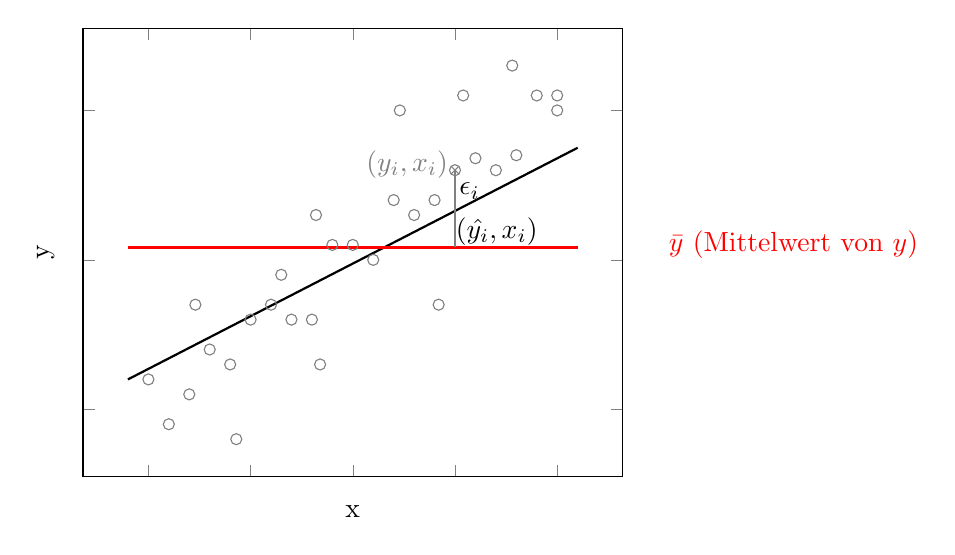
\begin{tikzpicture}
\begin{axis}[%
scatter/classes={%
	a={mark=o,draw=gray},
	b={mark=x, draw=gray}},
xlabel={x},
ylabel={y},
xticklabels={,,},
yticklabels={,,}
]
\addplot[scatter,only marks,%
scatter src=explicit symbolic]%
table[meta=label] {
	x y label
	10 12 a
	11 9 a
	12 11 a
	12.3 17 a
	13 14 a
	14 13 a
	14.3 8 a
	15 16 a
	16 17 a
	16.5 19 a
	17 16 a
	18 16 a
	18.2 23 a
	18.4 13 a
	19 21 a
	20 21 a
	21 20 a
	22 24 a
	22.3 30 a
	23 23 a
	24 24 a
	24.2 17 a
	25 26 a
	25 26 b
	25.4 31 a
	26 26.8 a
	27 26 a
	27.8 33 a
	28 27 a
	29 31 a
	30 30 a
	30 31 a
};
\addplot [thick] coordinates { (9,12) (31,27.5) };
\addplot [thick, red] coordinates { (9,20.83) (31,20.83) };

\addplot [gray] coordinates { (25,20.83) (25,26) };
\end{axis}

\node[red] at (rel axis cs:1.4,0.6){$\bar{y}$ (Mittelwert von $y$)};

\node[] at (rel axis cs:0.85,0.63){$(\hat{y_i},x_i)$};
\node[] at (rel axis cs:0.8,0.72){$\epsilon_i$};
\node[gray] at (rel axis cs:0.684,0.78){$(y_i,x_i)$};

\end{tikzpicture}


\[ \underbrace{\sum\limits_{i=1}^n (y_i - \bar{y})^2}_{\text{TSS (total sum of squares)}} = \underbrace{\sum\limits_{i=1}^n (\hat{y}_i - \bar{y})^2}_{\text{erklärbare Varianz}} + \underbrace{\sum\limits_{i=1}^n (\hat{y}_i - y)^2}_{\text{nicht erklärbare Varianz (RSS)} \epsilon_i = \hat{y}_i -y_i} \]

\subsection{Schätzung der Parameter $\beta_0$ und $\beta_1$}
Methode der kleinsten Quadrate: Reduziere Differenz zwischen Werten der Zielvariablen $y_i$ und den vorhergesagten Werten $\hat{y}_i$ für alle Beobachtungen $n$

\[ RSS = \sum\limits_{i=1}^n (y_i -\hat{y}_i)^2 \rightarrow min \]
\[ = \sum\limits_{i=1}^n (y_i -\hat{\beta_0} - \hat{\beta_1} x_i)^2 \rightarrow min \]
\[ \hat{\beta_1} = \frac{\sum\limits_{i=1}^n(x_i - \bar{x})(y_i - \bar{y})}{\sum\limits_{i=1}^n(x_i - \bar{x})} = 
\frac{Cor(X,Y)}{Var(X)} \]
\[ \hat{\beta_0} = \hat{y_i} - \hat{\beta_1}\bar{x} \]

%Vorlesung 8
\subsection{Güte der Schätzungen für $\beta_0$ und $\beta_1$}
Beachten Sie: Der wahre Zusammenhang zwischen $Y$ und $X$ ist unbekannt. D.h. die wahre Regressionsgerade ist unbekannt.\\
Grund: Schätzungen für $\hat{\beta_0}$ und $\hat{\beta_1}$ hängen von der gewählten Trainingsmenge ab. \\
Daraus folgt: 
\begin{itemize}
	\item Die geschätzten Regressionsgeraden schwanken um die wahre Regressionsgerade.
	\item Koeffizienten $\beta_0$ und $\beta_1$ sind Zufallsvariablen, welche auf Basis der gezogengen Beobachtungen $(x_i,y_i)$ geschätzt werden.
\end{itemize}

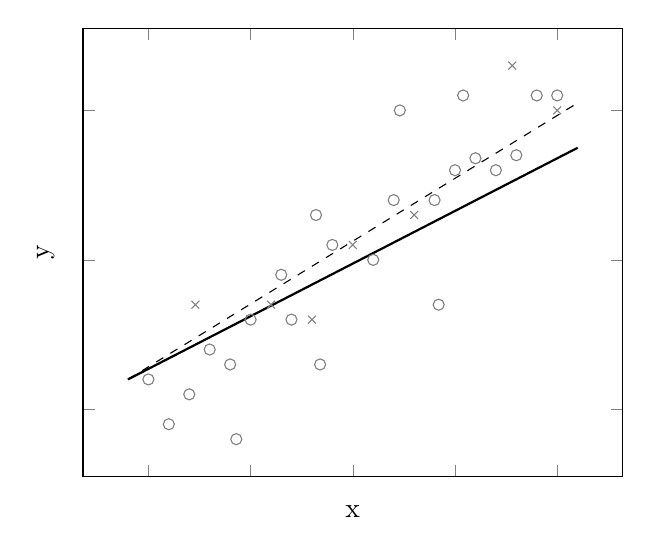
\begin{tikzpicture}
\begin{axis}[%
scatter/classes={%
	a={mark=o,draw=gray},
	b={mark=x,draw=gray}},
xlabel={x},
ylabel={y},
xticklabels={,,},
yticklabels={,,}
]
\addplot[scatter,only marks,%
scatter src=explicit symbolic]%
table[meta=label] {
	x y label
	10 12 a
	11 9 a
	12 11 a
	12.3 17 b
	13 14 a
	14 13 a
	14.3 8 a
	15 16 a
	16 17 b
	16.5 19 a
	17 16 a
	18 16 b
	18.2 23 a
	18.4 13 a
	19 21 a
	20 21 b
	21 20 a
	22 24 a
	22.3 30 a
	23 23 b
	24 24 a
	24.2 17 a
	25 26 a
	25.4 31 a
	26 26.8 a
	27 26 a
	27.8 33 b
	28 27 a
	29 31 a
	30 30 b
	30 31 a
};
\addplot [thick] coordinates { (9,12) (31,27.5) };
\addplot [dashed] coordinates { (9,12) (31,30.5) };
\end{axis}
\end{tikzpicture}

Varianz für $\beta_1$:
\[ Var(\beta_1)= \frac{\sigma_{\epsilon}^2}{\sum\limits_{i=1}^n (x_i-\bar{x})^2} \]
mit $\sigma_{\epsilon}^2$ ist die Varianz der Fehler $\epsilon$
\[\sigma_{\epsilon}^2 = \frac{RSS}{n-2} \]
\[\hat{Var}(\beta_1)=\frac{RSS/(n-2)}{\sum\limits_{i=1}^n (x_i-\bar{x})^2} \]
Varianz von $\beta_1$ ist klein, wenn:
\begin{enumerate}
	\item Varianz der Störgrößen klein ist
	\item Stichprobengröße $n$ groß ist
\end{enumerate}

\[ Var(\beta_0)= \frac{ \sigma_{\epsilon}^2 \sum x_i^2}{n Var(X)} \]

\subsection{Das Bestimmtheitsmaß $R^2$}
Wie gut ist die Schätzung der Daten anhand der gefitteten Geraden. \\
$\Rightarrow$ Schätzung ist dann besonders gut, wenn der Anteil von RSS an Gesamtvarianz(TSS) klein ist und somit die erklärte Varianz möglichst groß ist.

\[ R^2= \frac{\text{erklärbare Varianz}}{\text{Gesamtvarianz}}
= \frac{TSS-RSS}{TSS} = 1 - \frac{RSS}{TSS}\]
\todo{$TSS=\sum(\hat{y}-\bar{y})^2 + RSS$}

\[ 0 \leq R^2 \leq 1\]
$R^2 \approx 1$: Ein großer Anteil der Variabilität in der Zielvariablen durch gelernte Regressionsgerade erklärt. \\
$R^2 \approx 0$: \underline{Kein} großer Anteil der Variabilität in der Zielvariablen durch gelernte Regressionsgerade erklärt.

\subsection{Testen ob es einen signifikanten Zusammenhang zwischen $Y$ und $X$ gibt}
Frage: Existiert irgendein Zusammenhang zwischen $X$ und $Y$ gibt, also $\beta_1 \neq 0$. \\
$H_0$: Es existiert kein Zusammenhang $\Leftrightarrow \beta_1 = 0$ \\
$H_1$: Es existiert ein Zusamenhang $\Leftrightarrow \beta_1 \neq 0$ \\
Teststatistk: t-Statistik,welche t-Verteilung folgt \\
$ |t| \leq t_{1-\alpha/2} n-2  \Rightarrow H_0  \text{ wird beibehalten}$\\
$ |t| > t_{1-\alpha/2} n-2  \Rightarrow  H_0 \text{ abgelehnt } \Rightarrow \text{ Wir können annehmen }\beta_1 \neq 0$\\
\subsection{Multivariate lineare Regression}
\begin{enumerate}
	\item Erweiterung der einfachen linearen Regression auf mehreren Kovariablen $X=\{X_1,...,X_p\}$
	\item Identifiziere ein verbessertes Modell als auf Basis einer einzigen Kovariable möglich
	\item Individuelle Effekte von $X_i$ können durch partielle Regressionsgeraden modelliert werden
	\item Jede partielle Regressionsgerade enstpricht (modelliert) den Effekt einer Kovariablen $X_i$ während alle anderen Kovariablen $X_{j \neq i}$  ihren Mittelwert annehmen
\end{enumerate}

\subsection{Additives Multivariables lin. Regressionsmodell}
Annahme: Effekt einer Kovariablen $X_i$ auf $Y$ ist unabhängig von allen anderen Kovariablen.
\[Y = \beta_0 + \beta_1 X_1 + \beta_2 X_2 + ... + \beta_p X_p + \epsilon \]
$\beta_1 ... \beta_p$: Effekt der Kovariablen $X_1 ... X_p$ auf $Y$ \\
$p$: Anzahl der Kovariablen \\
$\beta_0$: Mittelwert von $Y$, falls alle Koeffizienten $\beta_j = 0$ \\
$\epsilon$: Fehler $\epsilon \sim N(0, \sigma^2)$


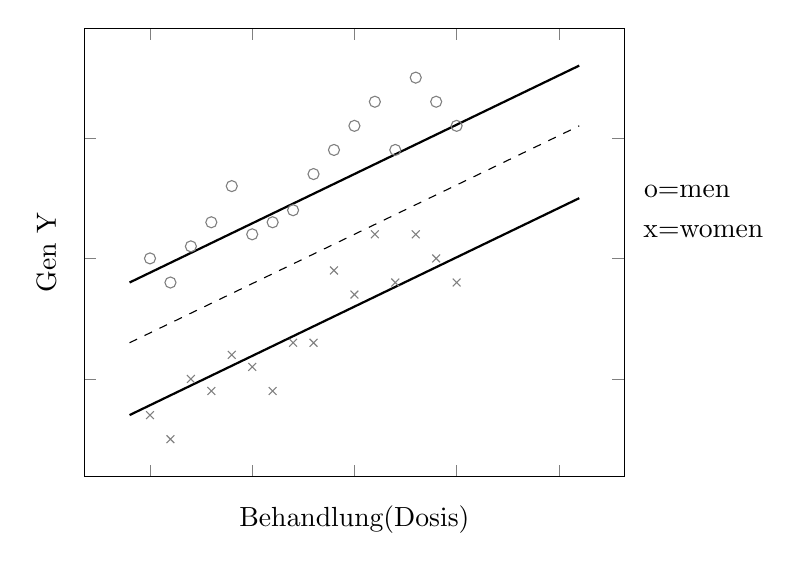
\begin{tikzpicture}
\begin{axis}[%
scatter/classes={%
	a={mark=o,draw=gray},
	b={mark=x,draw=gray}},
ylabel={Gen Y},
xlabel={Behandlung(Dosis)},
xticklabels={,,},
yticklabels={,,}
]
\addplot[scatter,only marks,%
scatter src=explicit symbolic]%
table[meta=label] {
	x y label
	10 20 a
	11 18 a
	12 21 a
	13 23 a
	14 26 a
	15 22 a
	16 23 a
	17 24 a
	18 27 a
	19 29 a
	20 31 a
	21 33 a
	22 29 a
	23 35 a
	24 33 a
	25 31 a
	10 7 b
	11 5 b
	12 10 b
	13 9 b
	14 12 b
	15 11 b
	16 9 b
	17 13 b
	18 13 b
	19 19 b
	20 17 b
	21 22 b
	22 18 b
	23 22 b
	24 20 b
	25 18 b
};
\addplot [thick] coordinates { (9,7) (31,25) };
\addplot [thick] coordinates { (9,18) (31,36) };
\addplot [dashed] coordinates { (9,13) (31,31) };
\end{axis}
\node[] at (rel axis cs:1.23,0.63){x=women};
\node[] at (rel axis cs:1.2,0.72){o=men};
\end{tikzpicture}
\todo{Hoher Fehler mit einfacher Regression (gestrichelt), also additiv nutzen}

\subsection{Multiplikatives Modell}
\begin{itemize}
	\item Interaktionen zwischen Kovariablen sind möglich
	\item D.h. partieller Effekt einer Kovariablen $X_i$ kann von partiellem Effekt von $X_j$ abhängig sein
\end{itemize}

\[Y = \beta_0 + \beta_1 X_1 + \beta_2 X_2 \beta_3 X_1 X_2 + ... + \beta_{p+1} X_p + \epsilon \]

$\beta_3$: Gibt an, inwieweit der Effekt von $X_1$ von den Werten von $X_2$ abghängt.

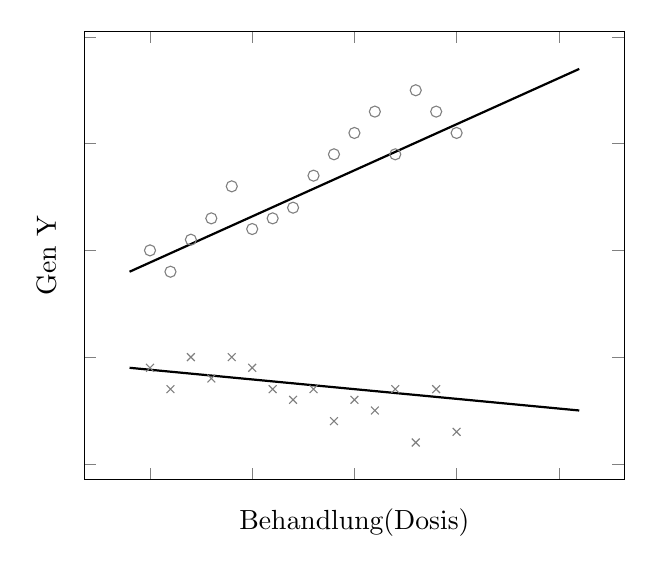
\begin{tikzpicture}
\begin{axis}[%
scatter/classes={%
	a={mark=o,draw=gray},
	b={mark=x,draw=gray}},
ylabel={Gen Y},
xlabel={Behandlung(Dosis)},
xticklabels={,,},
yticklabels={,,}
]
\addplot[scatter,only marks,%
scatter src=explicit symbolic]%
table[meta=label] {
	x y label
	10 20 a
	11 18 a
	12 21 a
	13 23 a
	14 26 a
	15 22 a
	16 23 a
	17 24 a
	18 27 a
	19 29 a
	20 31 a
	21 33 a
	22 29 a
	23 35 a
	24 33 a
	25 31 a
	10 9 b
	11 7 b
	12 10 b
	13 8 b
	14 10 b
	15 9 b
	16 7 b
	17 6 b
	18 7 b
	19 4 b
	20 6 b
	21 5 b
	22 7 b
	23 2 b
	24 7 b
	25 3 b
};
\addplot [thick] coordinates { (9,9) (31,5) };
\addplot [thick] coordinates { (9,18) (31,37) };
\end{axis}
\end{tikzpicture}

\subsection{Schätzung der Koeffizienten $\beta_1 ... \beta_p$}
Methode der kleinsten Quadrate
\[\hat{Y} = \hat{\beta_0} + \hat{\beta_1} X_1 + ... + \hat{\beta_p} X_p \]
\[ RSS = Var(\epsilon)= \sum\limits_{i=1}^n (y_i - \hat{y_i} )^2 \]
\[ \sum (y_i - \hat{\beta_0} - \hat{\beta_1} X_1 - ... - \hat{\beta_p} X_p )^2 \rightarrow min \]
Über partielle Ableitungen werden die Koeffizienten fpr $\beta_i$ geschätzt
